\Chapter{Introduction}
\label{chap:introduction}
	Solar energy is a prominent source of renewable energy across the globe. India has aimed to reach for 100 GW contribution from solar installations alone till 2022 \cite{mnreReport}. Silicon is the most preferred material for manufacturing the photovoltaic (PV) panels. This manufacturing process is energy intensive and thereby very costly. Extracting ingots from raw silicon accounts for 20\% of the total energy consumption throughout the process \cite{del09}. Hence, the initial cost of solar installation is higher. This can be reduced by finding better options for manufacturing silicon wafers.

\section{Methods for dicing silicon}
	The two popular methods for cutting of silicon are i) Wire loose slurry method and ii) Diamond saw cutting method. These methods, being abrasive in nature, lead to micro-fractures and cracks as deep as 20 $\mu$m in the final product. Because of this, the wafer size gets limited to 180 $\mu$m \cite{sopori13}. Also, about 50\% of the ingot material is lost as kerf losses \cite{joshi10}. These methods have other disadvantages like contamination of wafers due to slurry, etc. \cite{moeller2015}.

\subsection{Wire Loose Slurry Method}
	In this method, the workpiece is secured and a moving wire is used for cutting. The entire assembly is immersed in abrasive slurry to improve the cutting rate. The principle of operation of this technique is similar to that of a saw. The only difference is that slurry is used as abrasive material. This method is preferred for its improved processing time when multiple parallel wires are used on single ingot.

\subsection{Diamond Saw Cutting}
	A diamond coated abrasive wire is used in this method as opposed to the non abrasive wire from the previous method. This method can be used without any immersing medium. However, the assembly is usually immersed in water as diamond saw blades have been found to work better in wet conditions. Similar to the above method, multiple parallel abrasive wires are used in practice to improve the throughput of this process.

\subsection{Wire Electric Discharge Machining}
	WEDM is a novel machining process in which a moving thin wire electrode is used. Copper, tungsten, or brass wires with diameters of the order $10^{-4}$ m are commercially preferred. A small gap is always maintained between the work-piece and the wire. It is a through hole machining method capable to machine high strength and temperature resistance materials. Figure \ref{fig:lit-1} depicts the apparatus used for the experimentation hinted earlier, which schematically shows the arrangement in the actual WEDM machine.

	\begin{figure}[H]
		\centering
		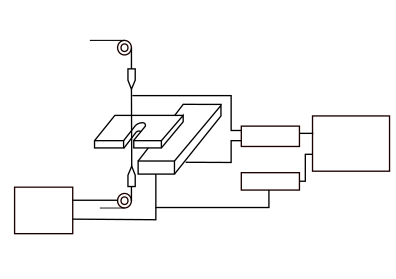
\includegraphics[width=0.8\textwidth]{wedm-diag}
		\caption{Diagrammatic representation of WEDM}
		\label{fig:lit-1}
	\end{figure}

	In WEDM, erosion of the workpiece material achieved by repetitive sparking in the gap between the work-piece and wire. Electrical energy from a pulsating DC power supply operating in the frequency range 0.5 to 30 kHz is used to generate the ionisation potential between the cathode and the anode at temperatures ranging from 8000$^\circ$ to 12000$^\circ$. Once turned off, plasma channel implodes, molten particles are flushed away and the gap recovers its dielectric strength. WEDM uses a fine wire travelling through the work-piece at a constant rate to avoid wire breakage due to formation of localised hotspots.

	%In the final product, a taper \cite{ho2004state} ranging from 15$^\circ$ for 100 mm thick to 30$^\circ$ for a 400 mm thick work-piece can be achieved. Typical Cutting Rates (CR) are 30 mm/min for 50 mm thick D2 tool steel and 750 mm/min for 150 mm thick aluminium.
	
	WEDM is a non contact micro-drilling process which can be used to cut free form contours from large solid metal workpieces. Experiments have shown that kerf width can be reduced from 250 $\mu$m in abrasive saw cutting to 50 $\mu$m in WEDM resulting in net material saving of 200 - 300\% \cite{dongre2015multi}. This method presents a promising alternative for application to silicon wafer manufacturing. Hence, the long term goal of this project is to optimise the manufacturing process of silicon wafers.

\section{Motivation}
	Although this process has been demonstrated for cutting of semiconductors and even ceramics \cite{sanchez2001development}, it is not as well established for these non conventional materials as it is for the metals. One reason for this is the lack of electrical characterisation of metal-semiconductor-dielectric sparks. The experimentation done to investigate this has so far led to the conclusion that the spark gap VI characteristics of silicon are very different from that of the steel \cite{kane2017aps}. Hence, it is important to find a reliable model for spark gap in this setting. However, the commercially available EDM machines are optimised for metals and have only discrete setting ranges. This has been acknowledged by \citet{levy1990wed}.

	Hence, the available machines are inadequate to carry out further experimentation as they provide discretely spaced setting ranges. An indigenously designed power supply along with a test setup is therefore required to carry out load investigations and optimise the process of Si-ingot cutting for PV applications.

\section{Scope}

	The goal of this project is to develop a pulsed power supply unit for WEDM which could deliver a variable ignition voltage and regulate the spark gap current. Such a regulated power supply is required for the experimentally understanding the WEDM process for silicon. The scope of this project extends to:
	\begin{itemize}
	\item Research of the existing pulsed power supplies is done to determine a suitable converter topology.
	\item Linear and  nonlinear modelling of the proposed supply.
	\item Controller design and verification via simulation for:\\
	1) Linear controllers: PI controller, current mode control, and compensator based control\\
	2) Nonlinear controller: Sliding mode control
	\item Design and fabrication of current and voltage sensing boards.
	\item Assembling the power circuit components with the digital signal processor.
	\item Implementing and hardware testing the PI controller.
	\end{itemize}

\section{Organisation of report}
	This report summarises the work done in design, modelling, and control of prototype power supply for Si-Ingot cutting by WEDM. Chapter \ref{chap:introduction} and \ref{chap:litreview} are dedicated to the introduction and the literature available on this regard.
	
	Chapter \ref{chap:modelling} describes the modelling process followed for deriving the dynamical models of the proposed power supply. In depth explanation of the time averaging technique of linear modelling and the direct technique for nonlinear modelling is provided here. The changes in system dynamics due to the deviation from the standard converter topology are also highlighted via the bode plots.

	The controller design of the aforementioned power supply is discussed in chapter \ref{chap:lincontrol}. The design procedures of linear controllers viz. PI controller, peak current mode control, and compensator based control form the first part of this chapter. This is followed by the theory and design of sliding mode controller.
	
	Chapter \ref{chap:hardware} is a detailed account of the hardware implementation of the pulsed power supply. This chapter describes the procedure followed for the selection of the passive components for the converter. The designs of sensor and interfacing boards, and the power circuit are described here.
	
	The simulation and the hardware experimentation results are included in the chapter \ref{chap:results}. This includes the simulation observations for the linear controllers and the hardware experimentation results with the PI controller. The current source time response is analysed in depth to reason out the observed behaviour. Towards the end of this chapter are the conclusions and the some possible future avenues that can be pursued.
	
	
